\section{Reference values}
\label{sec:reference}

Before the process is defined and its results derived, we collect in one place
the symbols, the key quantities, and the parameter combinations that will be
used throughout this chapter and the two that follow it. Everything listed here
is stated again, with derivation, in the body of the chapter; this page is the
reference card.

\newcommand\indentA{3cm}

\noindent
\textbf{Key parameters}
\begin{itemize}[leftmargin=\indentA]
\item[$\lambda$ :]birth rate (per replicative unit)
\item[$\mu$ :]death rate (per replicative unit)
\item[$\delta$ :]catastrophe rate (per replicative unit)
\end{itemize}

\noindent
\textbf{Defining quantities}
\begin{itemize}[leftmargin=\indentA]
\item[$\xt$ :]process state, the intracellular count
\item[$\xt=0$ :]internal extinction state (absorbing)
\item[$\xt=H$ :]catastrophe (rupture) state (absorbing)
\item[$\wt$ :]released count ($0$ before rupture, $\xx_{\tau^-}$ thereafter)
\item[$\tau$ :] catastrophe time
\item[$\Kb$ :]burst size, the value of $\xt$ immediately before rupture
\end{itemize}

\noindent
\textbf{Measures of stochasticity}
\begin{itemize}[leftmargin=\indentA]
\item[$I(t)$ :]$\pr{\xt\neq H}$, non-catastrophe probability
\item[$D(t)$ :]$p_0(t)=\pr{\xt = 0}$, probability of internal extinction (no burst)
\item[$\Ifix(t)$ :]$\pr{\xt\notin \{0,H\}} = I(t)-D(t)$, non-fixation probability (neither catastrophe nor death)
\item[$J(t)$ :]$\mean{\xt}$, expected process state
\item[$K(t)$ :]$\mean{\xt^2}$, second moment of the process state
\item[$V(t)$ :]$\mean{\wt}$, expected released count
\item[$p_n(t)$ :]$\pr{\xt = n}$, state probability distribution
\item[$P_k$ :]$\pr{\Kb = k}$, burst size distribution
\item[$\varphi(t)$ :]$\delta J(t)$, probability density of the burst time $\tau$ (defective when $\mu>0$)
\end{itemize}

\noindent
\textbf{Parameter combinations}
\begin{itemize}[leftmargin=\indentA]
\item[$\eta$ =]$\dfrac{\lambda+\mu+\delta}{2\lambda}$
\item[$a$ =]$\eta+\sqrt{\eta^2-\dfrac{\mu}{\lambda}}\quad(b<1<a)$
\item[$b$ =]$\eta-\sqrt{\eta^2-\dfrac{\mu}{\lambda}}$
\item[$A,B,\theta$ =]$a-1,\quad 1-b,\quad \lambda(a-b)$
\item[$\kappa$ =]$1+\dfrac{\delta}{2\lambda}$
\item[$w$ =]$\ee^{\theta t}$ (the recurring exponential of the closed forms)
\end{itemize}

\noindent
The constants $a$ and $b$ are the two roots of the quadratic
$\lambda x^2-(\lambda+\mu+\delta)x+\mu=0$, and $A$, $B$, $\theta$ measure
distances from the unstable root $1$. Their elementary identities, used
constantly in what follows, are
\begin{equation}
\label{eq:identities}
ab=\frac{\mu}{\lambda},\qquad a+b=\frac{\lambda+\mu+\delta}{\lambda},\qquad
AB=\frac{\delta}{\lambda},\qquad A+B=a-b,\qquad \theta=\lambda(a-b),
\end{equation}
each of which is immediate from Vieta's formulas together with the definitions
$A=a-1$ and $B=1-b$; they are re-derived in Section~\ref{sec:derivations}.

\begin{figure}[H]
\centering
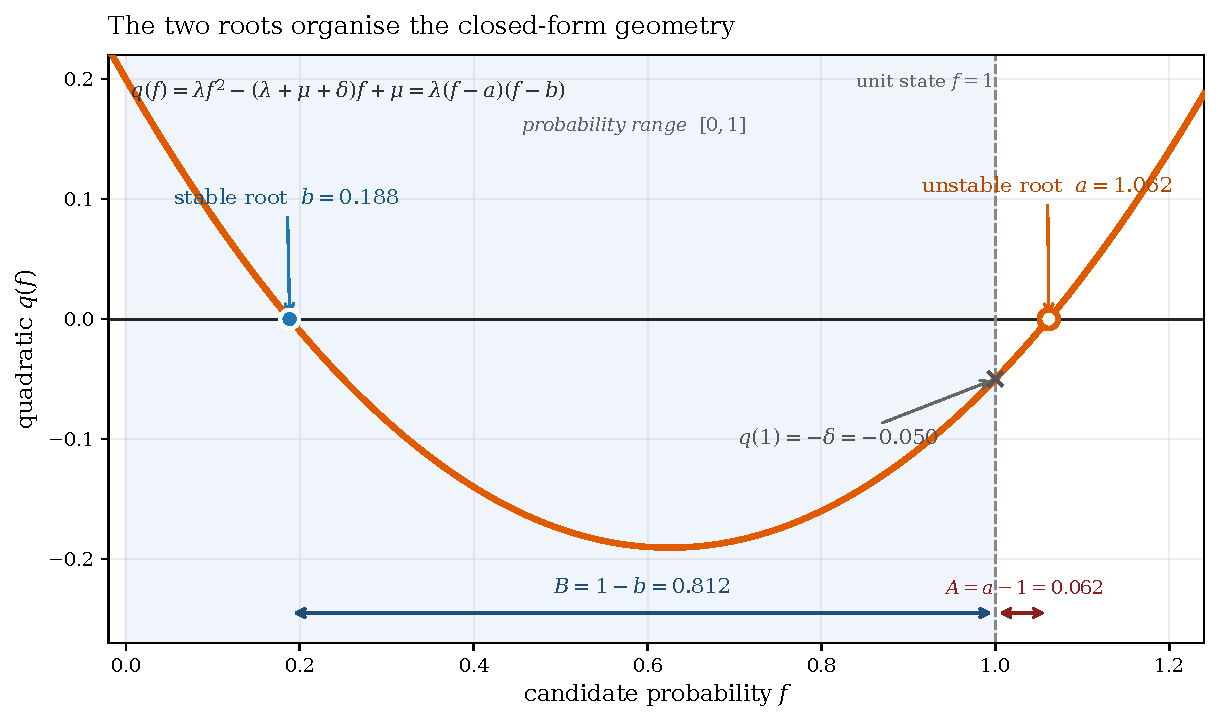
\includegraphics[width=0.72\textwidth]{figures/N3_4_quadratic_roots.pdf}
\caption{The characteristic quadratic for $\lambda=1$, $\mu=0.2$, and
$\delta=0.05$. Its roots are $b=0.188<1<a=1.062$; the distances
$B=1-b$ and $A=a-1$ set the geometric ratios and late-time constants used
throughout the chapter. Filled and open markers distinguish the stable and
unstable roots of the Riccati flow, respectively.}
\label{fig:N3_4}
\end{figure}

\noindent
\textbf{Key ODEs}
\begin{itemize}[leftmargin=\indentA]
\item[$\ddt{I}$]$ = \mu - (\lambda + \mu + \delta) I + \lambda I^2 = \lambda(I-a)(I-b)$ \\(Riccati equation for the non-rupture probability)
\item[$\ddt{I}$]$= -\delta J$ \\(forward equation for the rupture state)
\item[$\ddt{J} $]$= (\lambda - \mu)J - \delta K$ \\(expectation of $\xt$)
\item[$\ddt{V}$]$= \delta K $ \\(expectation of $\wt$)
\end{itemize}

\noindent
These four differential equations, together with the initial conditions
$I(0)=J(0)=K(0)=1$ and $V(0)=0$, generate every closed form derived in this
chapter.

\begin{figure}[H]
\centering
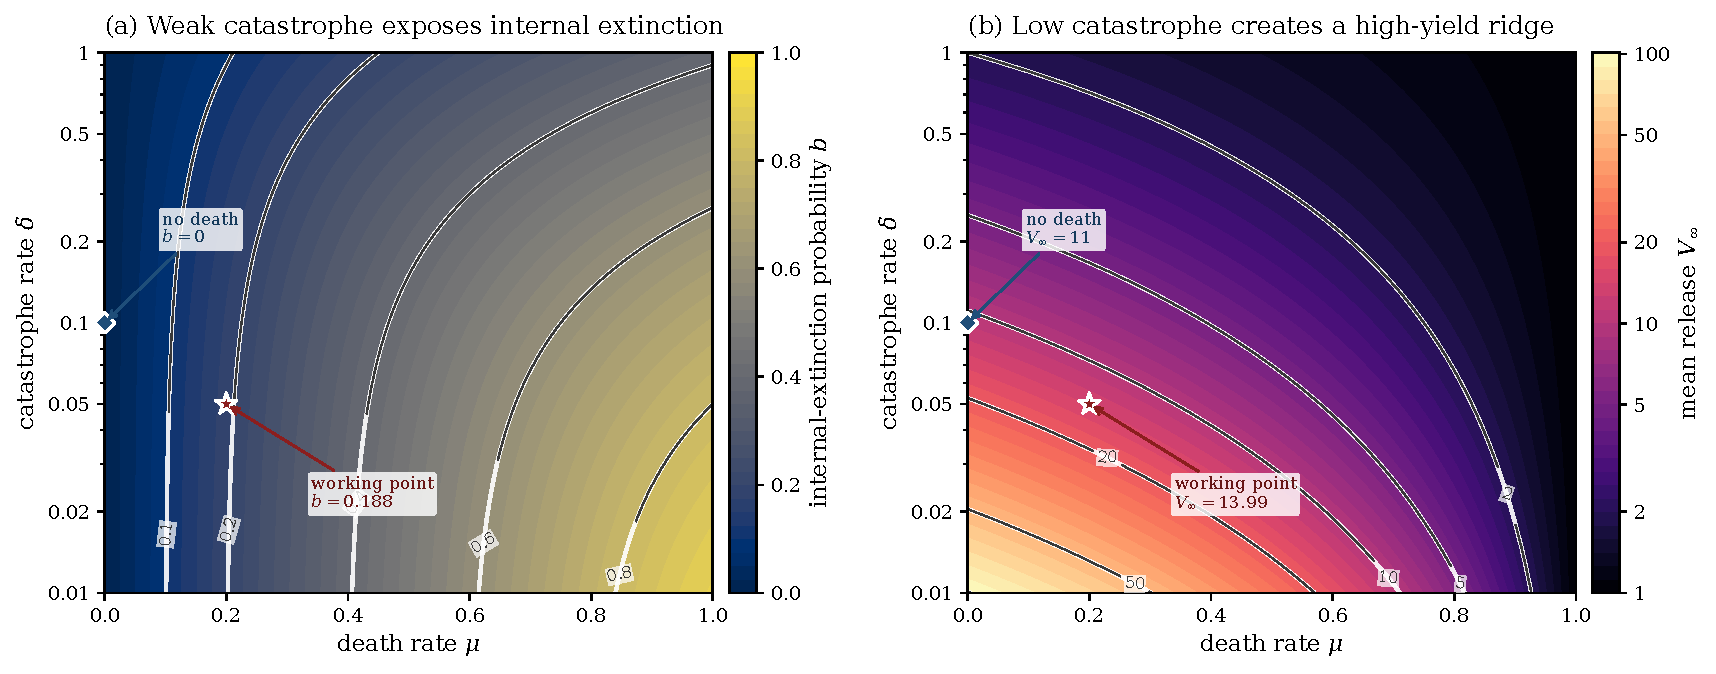
\includegraphics[width=0.98\textwidth]{figures/N3_7_b_Vinf_landscape.pdf}
\caption{Rate landscapes at fixed $\lambda=1$, shown for $\mu\in[0,1]$ and
$\delta\in[0.01,1]$ on a logarithmic $\delta$ axis. (a) The lower root $b$ is
the probability of internal extinction before release. (b) The mean release
$V_\infty$ forms a sharp high-yield ridge as catastrophe becomes rare. The
star marks the chapter's working point $(\mu,\delta)=(0.2,0.05)$, where
$b=0.188$ and $V_\infty=13.99$; the diamond marks the no-death point
$(0,0.1)$, where $b=0$ and $V_\infty=11$. Contours provide a
colour-independent reading of both landscapes.}
\label{fig:N3_7}
\end{figure}
